%\documentclass[handout]{beamer}
\documentclass{beamer}


% This file is a solution template for:

% - Giving a talk on some subject.
% - The talk is between 15min and 45min long.
% - Style is ornate.

\graphicspath{{images/}}


\mode<presentation>
{
  %\usetheme{Warsaw}
  %\usetheme{default}
  %\usetheme[secheader]{Madrid}
  \usetheme{Madrid}
  % or ...

  \setbeamercovered{transparent}
  % or whatever (possibly just delete it)
} 


\usepackage[english]{babel}
% or whatever

\usepackage[latin1]{inputenc}
% or whatever

\usepackage{times}
\usepackage[T1]{fontenc}
% Or whatever. Note that the encoding and the font should match. If T1
% does not look nice, try deleting the line with the fontenc.


% % % % % % MY COMMANDS % % % % % % % %

\newcommand{\tdot}[1]{\mathop #1\limits^{\bullet}}


\newcommand {\ux}{\underline{x}}

% % % % % % % % % % % % % % % % % % % % % % % % % %
\title[Lecture0 - Supplement]{Lecture0 - Supplement}





\date{Spring 2017}

\subject{Lecture}





% If you wish to uncover everything in a step-wise fashion, uncomment
% the following command: 

%\beamerdefaultoverlayspecification{<+->}




\mode<handout>
{
	\usepackage{pgf}
	\usepackage{pgfpages}
	
	\pgfpagesdeclarelayout{4 on 1 boxed}
	{
		\edef\pgfpageoptionheight{\the\paperheight} 
		\edef\pgfpageoptionwidth{\the\paperwidth}
		\edef\pgfpageoptionborder{0pt}
	}
	{
		\pgfpagesphysicalpageoptions
		{%
			logical pages=4,%
			physical height=\pgfpageoptionheight,%
			physical width=\pgfpageoptionwidth%
		}
		\pgfpageslogicalpageoptions{1}
		{%
			border code=\pgfsetlinewidth{2pt}\pgfstroke,%
			border shrink=\pgfpageoptionborder,%
			resized width=.5\pgfphysicalwidth,%
			resized height=.5\pgfphysicalheight,%
			center=\pgfpoint{.25\pgfphysicalwidth}{.75\pgfphysicalheight}%
		}%
		\pgfpageslogicalpageoptions{2}
		{%
			border code=\pgfsetlinewidth{2pt}\pgfstroke,%
			border shrink=\pgfpageoptionborder,%
			resized width=.5\pgfphysicalwidth,%
			resized height=.5\pgfphysicalheight,%
			center=\pgfpoint{.75\pgfphysicalwidth}{.75\pgfphysicalheight}%
		}%
		\pgfpageslogicalpageoptions{3}
		{%
			border code=\pgfsetlinewidth{2pt}\pgfstroke,%
			border shrink=\pgfpageoptionborder,%
			resized width=.5\pgfphysicalwidth,%
			resized height=.5\pgfphysicalheight,%
			center=\pgfpoint{.25\pgfphysicalwidth}{.25\pgfphysicalheight}%
		}%
		\pgfpageslogicalpageoptions{4}
		{%
			border code=\pgfsetlinewidth{2pt}\pgfstroke,%
			border shrink=\pgfpageoptionborder,%
			resized width=.5\pgfphysicalwidth,%
			resized height=.5\pgfphysicalheight,%
			center=\pgfpoint{.75\pgfphysicalwidth}{.25\pgfphysicalheight}%
		}%
	}
	
	
	\pgfpagesuselayout{4 on 1 boxed}[a4paper, border shrink=5mm, landscape]
	\nofiles
}


\begin{document}

\begin{frame}
  \titlepage
%  \begin{figure}
%	\centering
%		\includegraphics[width=1.5cm]{images/Picture1} \ \ \ \
%		\includegraphics[width=1.5cm]{images/Picture2}
%	\label{fig:Picture11}
%\end{figure}
\end{frame}

%\begin{frame}{Outline}
%  \tableofcontents
%  % You might wish to add the option [pausesections]
%\end{frame}

\section{What is an image?}

\begin{frame}%<handout:0>

\textbf{What is an image?}	

\

\begin{enumerate}
	\item Ideally, we think of an \textbf{image} as a 2-dimensional light intensity function, 
	$f(x,y)$, where $x$	and $y$	are spatial coordinates, and $f$ at $(x,y)$
	is related to the brightness or colour of the image at that point.
	
	\item  In practice, most images are defined over a rectangle.
	
	\item Continuous in amplitude ("continuous-tone").
	
	\item Continuous in space: no pixels!
\end{enumerate}
	
\end{frame}

\begin{frame}<handout:0>
	
	\begin{center}
		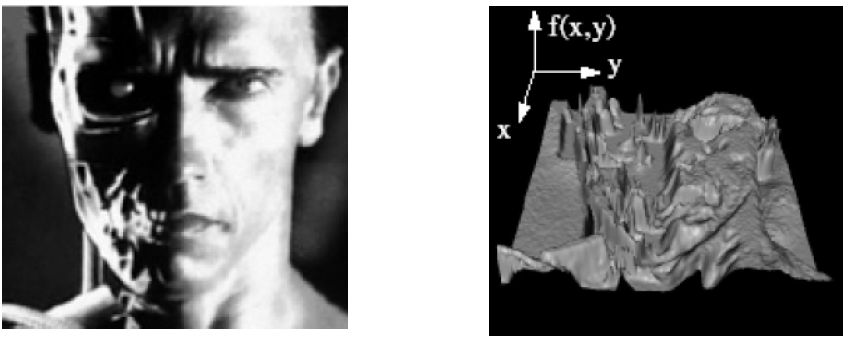
\includegraphics[width=12cm]{./images/termin.jpg} 
	\end{center}
\end{frame}

\begin{frame}%<handout:0>
\textbf{Digital Images and Pixels}	

\

\begin{enumerate}
	\item A \textbf{digital} image is the representation of a continuous image 
	f(x,y)
	f(x,y)
	by a 2-d array of discrete samples. The amplitude of each sample is quantized to be represented by a finite number of bits.
	
	\
	
	
	\item Each element of the 2-d array of samples is called a pixel or pel (from "picture element").
	
	
		
\end{enumerate}
\end{frame}

\begin{frame}<handout:0>
\textbf{	A Digital Image is Represented by Numbers}

\
	
	\begin{center}
		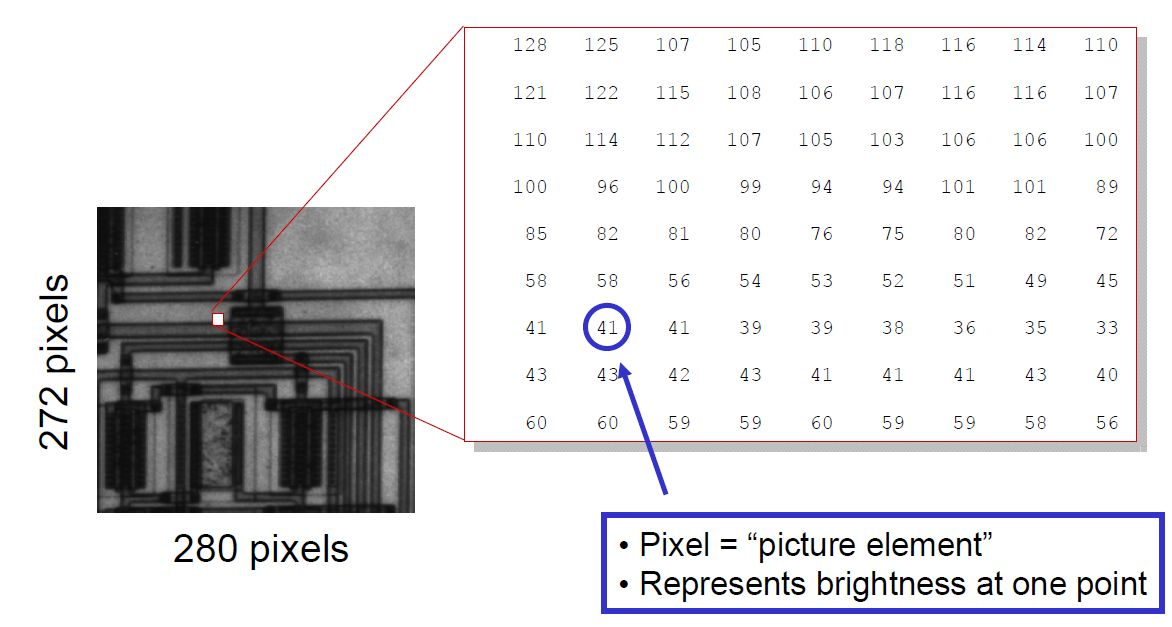
\includegraphics[width=12cm]{./images/pixel_example.jpg} 
	\end{center}
\end{frame}


\begin{frame}%<handout:0>
	\textbf{A digital image can be represented as a matrix}
	
	Coordinate convention used in this course to represent digital images (Matlab uses another convention). 
	
	\
	
	\begin{center}
		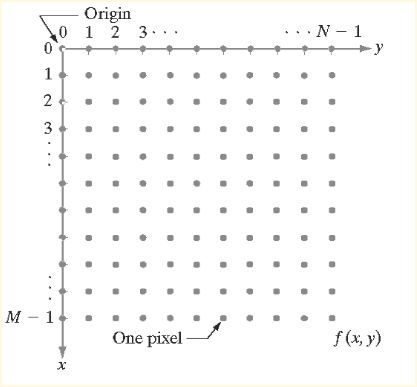
\includegraphics[width=6cm]{./images/coordinate_example.jpg} 
	\end{center}
\end{frame}


\begin{frame}%<handout:0>
	
%	{\textbf{A digital image can be represented as a matrix}}
	
	
	The notation introduced in the preceding slide allows us to write the 
	complete $M \times N$ digital image in the following compact matrix form: 
	
	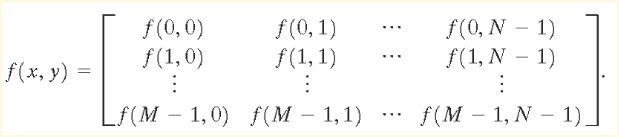
\includegraphics[scale = 0.4]{./images/matrix_example.jpg}
	
	\
	
	In some discussions, it is advantageous to use a more traditional matrix no- 
	notation to denote a digital image and its elements: 
	
	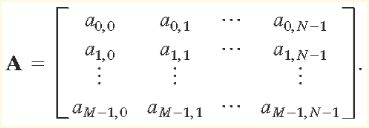
\includegraphics[scale = 0.4]{./images/matrix1_example.jpg}
	
	The sampling process may be viewed as partitioning the $xy$ plane into a grid, with the coordinates of the center of each grid. For a colour image, $f$
	might be one of the components.
	
\end{frame}







\begin{frame}<handout:0>
	
	{\textbf{Colour Components}}
	
	
	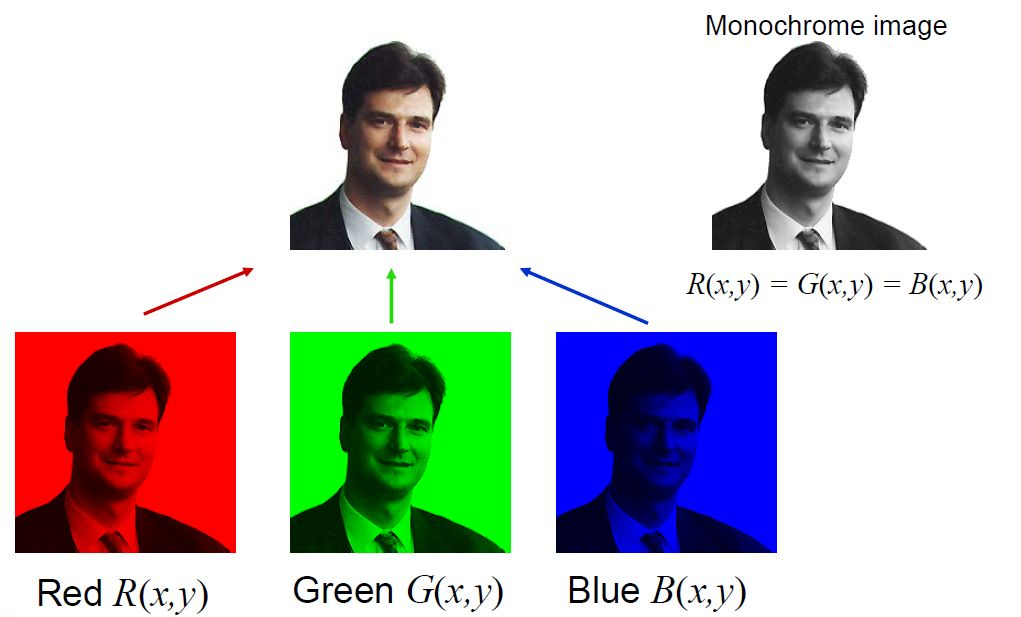
\includegraphics[scale = 0.3]{./images/colour4_example.jpg}
\end{frame}


\begin{frame}
	
	{\textbf{Different numbers of gray levels}}
	
	
	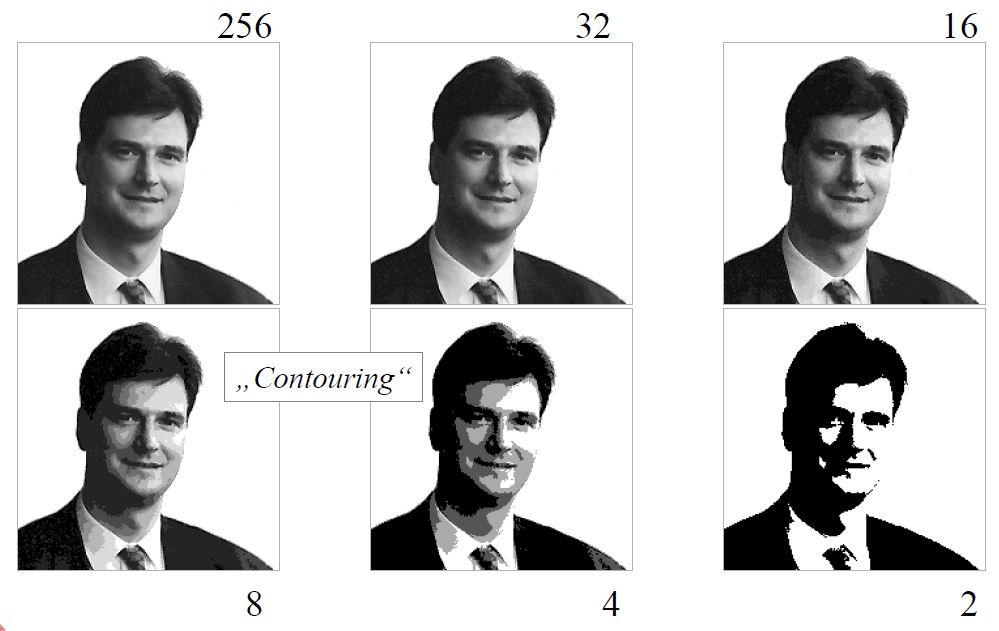
\includegraphics[scale = 0.3]{./images/gray1_example.jpg}
\end{frame}


\begin{frame}
	
	{\textbf{How many gray levels are required?}}
	
	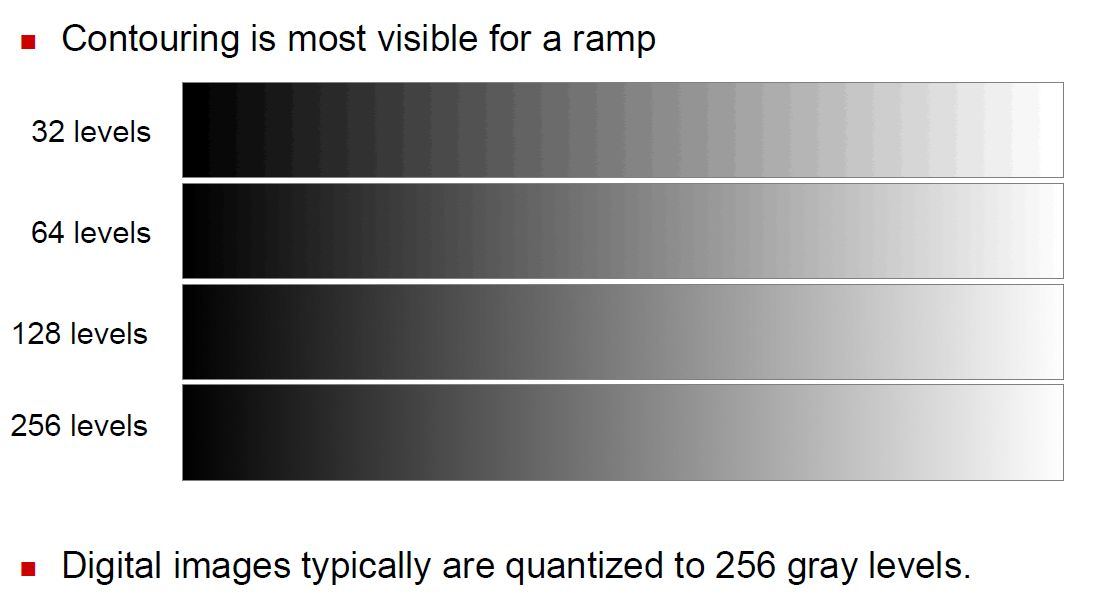
\includegraphics[scale = 0.3]{./images/gray2_example.jpg}
\end{frame}





\begin{frame}<handout:0>
\textbf{	Image Manipulation with Python (Matplotib Library)}
\end{frame}
\end{document}

%%%%%%%%%%%%%%%%%%%%%%%%%%%%%%%%%%%%%%%%%%%%%









% % % % % % % % % % % % % % % % % % % % % % % % % % % % % % % % % % % % % % % % % % %

\begin{frame}%<handout:0>
	
\end{frame}

% this frame won't be included in the handout mode
\begin{frame}<handout:0>
	I am a lolcat!
\end{frame}



To add to the suggestions above, to disable the frame in both handout and beamer modes, one must add

<handout:0|beamer:0>

